\section{Background}\label{sec-background}
In this section, we briefly overview the current challenges with view maintenance and
our prior work in scalable data cleaning.

\begin{figure}[ht!] 
\centering
\vspace{-0.75em}
 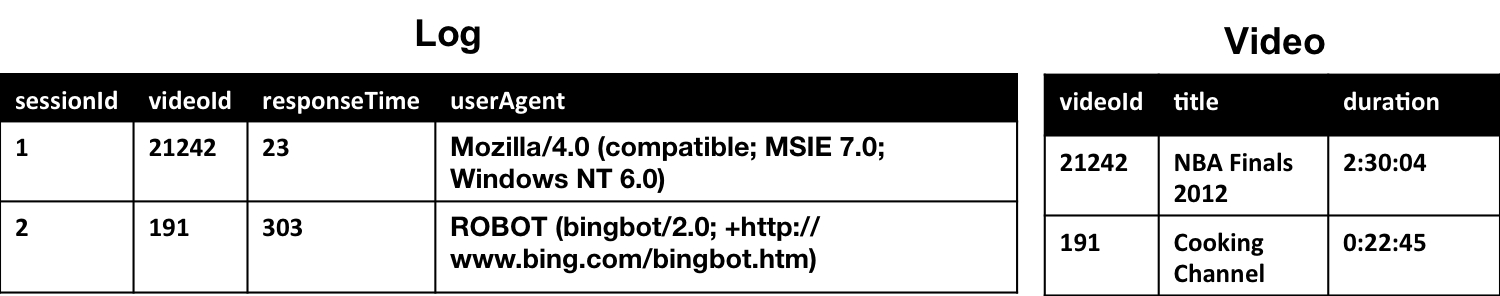
\includegraphics[width=\columnwidth]{figs/sample-clean-example.png}\vspace{-0.25em}
 \caption{A simplified log analysis example dataset. In this dataset, there are two tables: a fact table representing video views and a dimension table representing the videos.\label{example-1}}
\end{figure}

\subsection{Running Example: Log Analysis}
To illustrate our system, we use the following running example which is a 
simplified schema of one of our experimental datasets (Figure~\ref{example-1}).
Imagine, we are querying logs from a video streaming company. 
These logs record visits from users as they happen and grow over time.
We have two tables, \tbl{Log} and \tbl{Video}, with the following schema:

\begin{lstlisting}[mathescape]
Log(sessionId$\textrm{,}$ videoId$\textrm{,}$ responseTime$\textrm{,}$ userAgent)
Video(videoId$\textrm{,}$ title$\textrm{,}$ duration)
\end{lstlisting}
These tables are related with a foreign-key relationship between
Log and Video.
Though SVC supports inserts, deletions, and updates, for clarity in our example, we consider insertions
into Log which is cached in a temporary table:
\begin{lstlisting}[mathescape]
LogInserts(sessionId$\textrm{,}$ videoId$\textrm{,}$ responseTime$\textrm{,}$ userAgent)
\end{lstlisting}

\subsection{Materialized View Maintenance}\label{subsec-inc}
Views define logical relations which can be queried instead of physical base relations.
Materialized views are a class of views that are pre-computed and stored (i.e materialized).
Any form of pre-computed, derived data encounters the problem of staleness when the physical base relations changes.

One approach to this problem is to recompute the materialized view every time there are updates to the base tables.
However, this approach is very inefficient if updates to the data generally have small or sparse effect on the materialized view. 
A contrasting approach is incremental view maintenance (IVM), where rows in the materialized views are incrementally updated based on the updates to the base table.
Incremental maintenance of materialized views has been well studied; see \cite{chirkova2011materialized} for a survey of the approaches. 
At a high-level, incremental maintenance algorithms typically consist of the following steps: (1) maintain a cache of insertions and deletions for each physical base table, then using the view definition derive a \emph{change propagation formula} in terms of the set of insertions and deletions, and finally apply the formula to the materialized view.
For a variety of view types, these rules are described in detail in \cite{DBLP:journals/vldb/KochAKNNLS14, DBLP:conf/pods/Koch10}.

Incremental maintenance may not be efficient in all cases.
Consider the view that calculates the median responseTime grouped by userAgent on our running example dataset.
In general, to ensure correctness, the view has to store the entire set of responseTime attributes for each group to allow for incremental maintenance.
Along the lines of this example, there are cases when recomputation may require less storage of state or even less computation.
Thus, materialized views are maintained either with incremental maintenance, recomputation, or a mix.

\subsubsection{Practical Considerations}
The algebraic analysis of incremental maintenance \cite{DBLP:journals/vldb/KochAKNNLS14, DBLP:conf/pods/Koch10} informs us which views can be incrementally maintained efficiently.
However, there are many practical considerations of excuting these operations in real database systems and it may not always be feasible to immediately apply updates; even if theoretically possible.
The main problem is that while immediate incremental maintenance has many advantages, the particulars of the database system and available resources often dictate how updates are propagated.

To address these challenges, deferred maintenance is an alternative and often preferred solution.
The main insight of deferral is to avoid maintaining the view immediately and to schedule an update at a more convenient time either in a pre-set way or adaptively.
In deferred maintenance approaches, the user often accepts some degree of staleness for additional flexibility in scheduling.
These costs can also be deferred to query execution time.
In particular, we highlight a technique called lazy maintenance which applies updates to the view only when a user's query requires a row \cite{zhou2007lazy}.
While always fresh, both lazy maintenance and immediate maintenance hit a bottleneck when there are rapid updates, and this results increasingly degraded performance if a user wants to query a view.
The alternative is a periodic strategy, but this means that there is unbounded error on queries between maintenance periods.

The data cleaning perspective that SVC offers on this problem is that there is a tradeoff between accuracy and computation.
By using sampling, we give the user access to a new tradeoff space between immediate (or close to immediate, i.e., mini-batch) maintenance and long-periodic maintenance.

\subsection{SampleClean: Fast and Accurate Query Processing on Dirty Data}
In our prior work on the SampleClean project \cite{wang1999sample}, we proposed a framework for scalable data cleaning.
Similar to the accuracy-performance contrast between incremental maintenance and periodic maintenance in the materialized view setting, data cleaning also faces a similar challenge.
Traditionally, data cleaning has explored expensive, up-front cleaning of entire datasets for increased query accuracy, and those who were unwilling to pay the full cleaning cost avoided data cleaning altogether.
We proposed SampleClean to add an additional tradeoff to this design space by using sampling.

SampleClean (Figure \ref{sc}) has three parts: (1) sampling, (2) data cleaning, and (3) query result estimation.
First, SampleClean creates a sample of dirty data (which are erroneous, missing, or otherwise corrupted records).
Then, the framework applies a data cleaning operation to the sample.
Finally, when users query the dataset, the framework uses the clean sample to extrapolate clean query results.
The key challenge is that data cleaning can potentially change the statistics of a sample and the queries need to compensate for those effects.
In our initial work, SampleClean focused on three common aggregates: \sumfunc, \avgfunc, and \countfunc queries.

In SampleClean, we noticed that there were two contrasting query processing approaches, which we termed: \textbf{RawSC} \reminder{Define new commands for RawSC and NormarlizedSC. I would suggest to use \textsf{RawSC} instead of \textbf{RawSC}} and \textbf{NormalizedSC}.
In \textbf{RawSC}, we could apply queries, with some re-weighting, directly to the clean sample of data.
This approach is very similar to that taken in Sample-based Approximate Query Processing \cite{OlkenR86,AgarwalMPMMS13, joshi2008materialized}.
\textbf{NormalizedSC}, on the other hand, processed the changes made by the data cleaning and issued ``corrections" to the query results.
We found that these two algorithms tradeoff statistical efficiency and robustness to error; as \textbf{RawSC} only depends on clean data it is robust to the magnitude of data error and as \textbf{NormalizedSC} depends on the delta of the data cleaning it performs well when the data cleaning is sparse. 
In this work, we found that estimating a correction (\textbf{NormalizedSC}) led to lower variance results on real datasets (see Section \ref{exp}). 

\begin{figure}[t] \vspace{-2em}
\centering
 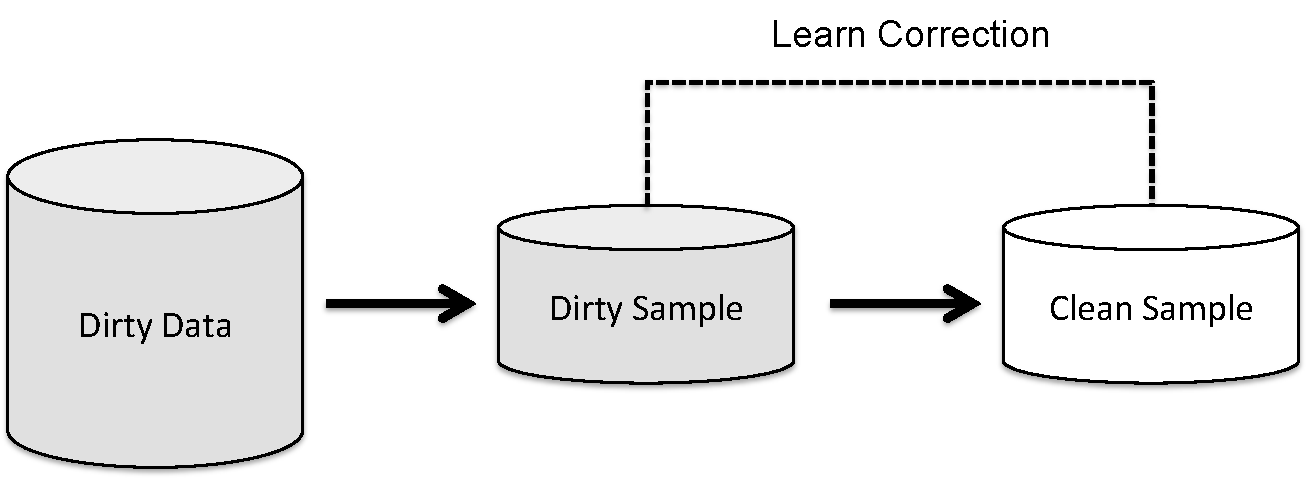
\includegraphics[scale=0.30]{figs/sys-arch2.pdf} \vspace{-.25em}
 \caption{A basic overview of SampleClean. SampleClean uses a random sample of dirty data to learn how a data cleaning algorithm affects queries on the sample. We can then derive a correction to compensate for the dirtiness.  \label{sc} \reminder{This only shows NormalizedSC}}\vspace{-1.75em}
\end{figure}

\subsection{New Challenges}
Inspired by SampleClean, SVC samples a stale view, cleans the sample view by restricting the maintenance to just the rows in the sample, and then applies \textbf{NormalizedSC} to correct the results of queries on the view.
Applying this data cleaning framework to the materialized view setting leads to some interesting theoretical challenges with new insights for both materialized view maintenance and data cleaning.
In materialized views, unlike the models of error studied in SampleClean, staleness can lead to rows that are missing from the ``dirty" view or conversely need to be deleted.
This problem poses an important statistical challenge since to calculate a correction with \textbf{NormalizedSC} we need to measure the difference in rows attribute values after cleaning, and this requires us to define this algorithm when rows are missing from either side of the difference.
In SampleClean, we also assumed samples were derived directly from base relations.
However, efficiently sampling from materialized views is much more complex.

We further use this new setting to explore and formalize the class of queries that our frameworks can support.
We extend the generality of the framework to support queries than the \sumfunc, \avgfunc, and \countfunc which studied before.
We show that \textbf{NormalizedSC} actually can give meaningful results for some \selectfunc queries.
A further insight is that queries without closed form confidence intervals can also be supported, and we
derive an algorithm to achieve empirical confidence intervals for aggregates such as \texttt{median} and \texttt{corr}.

Sampling is particularly sensitive to variance in the dataset, and large outliers can significantly reduce query accuracy.
In this work, we give an explicit treatment of non-erroneous outliers records.




